\documentclass[aspectratio=169]{beamer}
\usepackage{beamerthemesidebar}
\usepackage{hyperref}
\usepackage{color}
\usepackage{multimedia}
\usepackage{colortbl}
\usepackage{amsmath}
\usepackage{empheq}
\usepackage{cancel}
\usepackage{amssymb}
\usepackage{amsfonts}
\usepackage{lipsum}
\usepackage{tcolorbox}
\usepackage{tabularx}
\usepackage{caption}

\setbeamersize{sidebar width right=0pt}
\setbeamertemplate{footline}[frame number]
%
\definecolor{orange}{RGB}{250,167,12}
\definecolor{yellow}{RGB}{246,250,12}
\definecolor{green}{RGB}{128,238,1}
\definecolor{black}{RGB}{0,0,0}
\definecolor{blue}{RGB}{0,0,255}
\definecolor{red}{RGB}{255,0,0}
\definecolor{sepia}{RGB}{94,38,18}
\newcommand{\ve}[1]{{\rm\bf {#1}}}
\newcommand{\q}[1]{\textcolor{blue}{#1}}
\newcommand{\blue}[1]{\textcolor{blue}{#1}}
\newcommand{\sepia}[1]{\textcolor{sepia}{#1}}
\newcommand{\red}[1]{\textcolor{red}{#1}}
\newcommand{\green}[1]{\textcolor{green}{#1}}
\newcommand{\yellow}[1]{\textcolor{yellow}{#1}}
\newcommand{\orange}[1]{\textcolor{orange}{#1}}
\definecolor{burlywood}{RGB}{255,211,155}
\definecolor{chocolate}{RGB}{255,127,36}
\definecolor{tan}{RGB}{210,180,140}
%
%
\title{Theoretical Astrophysics I: Stellar Structure and Evolution\\
Lecture 1: Course Introduction and History of stellar research}
\author{\texorpdfstring{\sepia{Petri K\"{a}pyl\"{a} Ivan Mili\'{c}}\newline\blue{\url{pkapyla, milic@leibniz-kis.de}}}{}}
\institute{Institut f\"ur Sonnenphysik - KIS, Freiburg}
\date{\today}
%
\begin{document}
\frame{\titlepage}

\section{Course organization and curriculum}
\frame{
\frametitle{Why study the stars?}
	\begin{itemize}
		\item The aim of this course is to show you how the stars ``work''. That is, what physical principles determine their structure, evolution, observable characteristics and phenomena taking place inside. 
		\item It is a mostly theoretical / computational course - but we will make connections to the observables (today, for example).
		\item Stars are building blocks of the universe (stars make up galaxies, which make up the large-scale structure).
		\item Stars generate magnetic fields, host planets, create elements heavier than Helium, trigger creation of other stars - and are, in general, very cool thing to research.
		\item The Sun is a special star which gives Earth \emph{a lot} of energy, determines the space weather conditions and gives us insight into how other stars function.
	\end{itemize}
}
%
\frame{
\frametitle{Who are we and what do we do?}
	\begin{itemize}
		\item We come from Institute for Solar Physics - KIS.
		\item KIS conducts fundamental research on the Sun and similar(ish) stars, develops instruments and computer codes and operates telescopes and the science data center (SDC).
		\item In practice, our institute works mostly on:
		\begin{itemize}
			\item High-resolution observations of the solar ``surface'' phenomena. 
			\item Diagnosing physical properties of the solar surface, most importantly the magnetic fields.
			\item Understanding the convection in Sun and other stars. 
			\item Studying solar and stellar interiors and surface phenomena using numerical simulations.
		\end{itemize}
		\item And the two of us... \q{Present and discuss 5 mins}.
	\end{itemize}
}
%
%
\frame{
\frametitle{How will this course work}
	\begin{itemize}
		\item Lectures once per week (2 $\times$ 45 min): 12 lectures + 1 general practice session at the end, before the exam.
		\item Hands-on exercises once per week (1 $\times$ 45 min): calculations / derivations on the blackboard or numerical calculations / data manipulation in \emph{python}
		\item 4-5 Homeworks (HW) covering similar material to handson. You will have 2-weeks per homework.
		\item So, it would be good if you had an access to a computer, in order to complete the HW. Would be nice to type it up and send it as pdf. Reach out if there are issues. 
	\end{itemize}
}
%
\frame{
\frametitle{Grading}
	\begin{itemize}
		\item Homework - 40\%
		\item Bonus problems in the homework - 10\% 
		\item Final exam - 60\%
		\item That's right - you can score more than 100\% - this gives you some flexibility. 
		\item There is no ``curve grading''.
		\item Whenever there is an issue - ask. You can reach out to us via e-mail or even phone :-)
	\end{itemize}
}
%
\frame{
\frametitle{Literature/materials}
	\begin{itemize}
		\item ``An introduction to the theory of stellar structure and evolution'', Dina Prialnik, 2007, CUP
		\item ``The Sun: an introduction'', Michael Stix, 2002, Springer
		\item When needed: research papers and texts. It would be good to familiarize yourself with some services:
		\item One is \href{https://ui.adsabs.harvard.edu/}{ADS} - a searchable database of astronomical papers
		\item The other is \href{https://github.com/}{github} - a repository for codes
		\item Finally, there is \href{https://www.overleaf.com/}{overleaf} - an online manuscript editor / manager
	\end{itemize}
}
%
\frame{
\frametitle{To summarize}
	\begin{itemize}
		\item Whatever you can't find, are unsure about, or don't understand - ask! 
		\item The goal is to learn new things and hopefully have some fun. 
		\item You are welcome to come see our institute, talk to us about science, ask us for research projects, etc.
		\item \q{Do you have any questions? (Use this time to collect the contacts and establish a mailing list)}.
		\item \q{Note: currently KIS gitlab is acting out}. Slides are \href{https://github.com/ivanzmilic/taipss}{at a public github}.
	\end{itemize}
}
%
\section{General astrophysical concepts}
\frame{
\frametitle{Astrophysics}
	Astrophysics is (literally) physics of stars. It also studies: planets, small bodies, galaxies, interstellar and intergallactic medium, etc. It gives us an opportunity to apply almost all fields of physics, to understand these specfic objects. It involves concepts from many other sciences:
	\begin{itemize}
		\item Physics: quantum, atomic, molecular, nuclear, thermodynamics, fluid dynamics, magnetohydrodynamics, relativity. 
		\item Chemistry, biology.
		\item Applied mathematics, optics, photonics, solid state (detectors, etc).
		\item Also involves/overlaps with: cosmology, celestial mechanics, particle physics...
	\end{itemize}
}

\frame
{
\frametitle{Uniqueness of astrophysics}
\begin{minipage}{0.48\linewidth}
\begin{itemize}
\item In the lab we can control the parameters of the experimental set-up to see
how results change.
\item In astrophysics this is impossible. We can only observe. Some of the first objects we observed were the Sun and stars.
\item But the physical laws are universal: what we learn through theory, experiment and observations is applicable everywhere.
\item There is also such thing as ``laboratory astrophysics'' - \q{What do you think that is? (1-2  mins)}
\end{itemize}
\end{minipage}
\hfill
\begin{minipage}{0.48\linewidth}
\begin{figure}
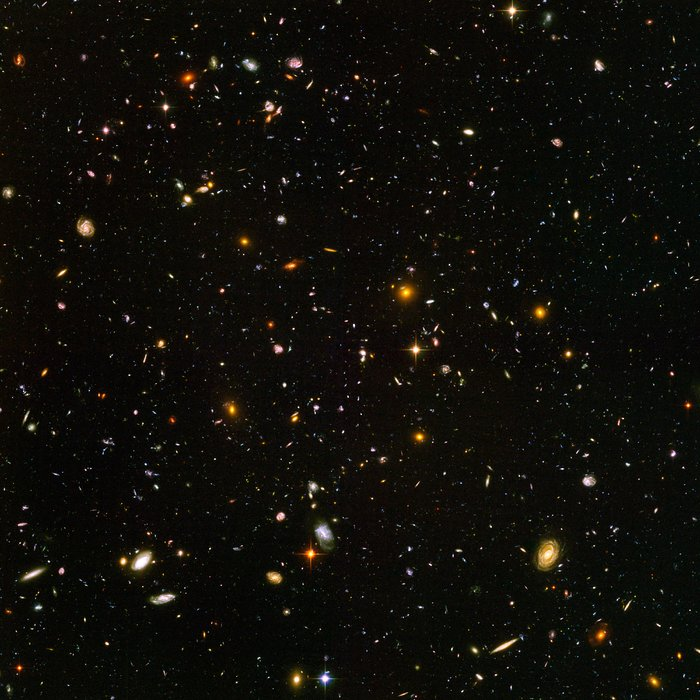
\includegraphics[width=5cm]{../figures/hubble_udf.jpg} \\
\caption*{Hubble Ultra Deep Field: credits to NASA}
\end{figure}
\end{minipage}
}
%
\frame{
\frametitle{Numerical experiments}
\begin{minipage}{0.48\linewidth}
\begin{itemize}
\item There are also \emph{numerical} experiments. 
\item We know, for hundreds of years, that most equations cannot be solved analytically.
\item They are not pecularities, they describe real-life problems. \q{Can you come up with any?}
\item To solve these, we use numerical simulations. These are computer codes that solve systems of integral and differential equations, and try to describe the structure and evolution of the objects.
\end{itemize}
\vspace{-0.25cm}
\end{minipage}
\hfill
\begin{minipage}{0.48\linewidth}
\begin{figure}
% herehere
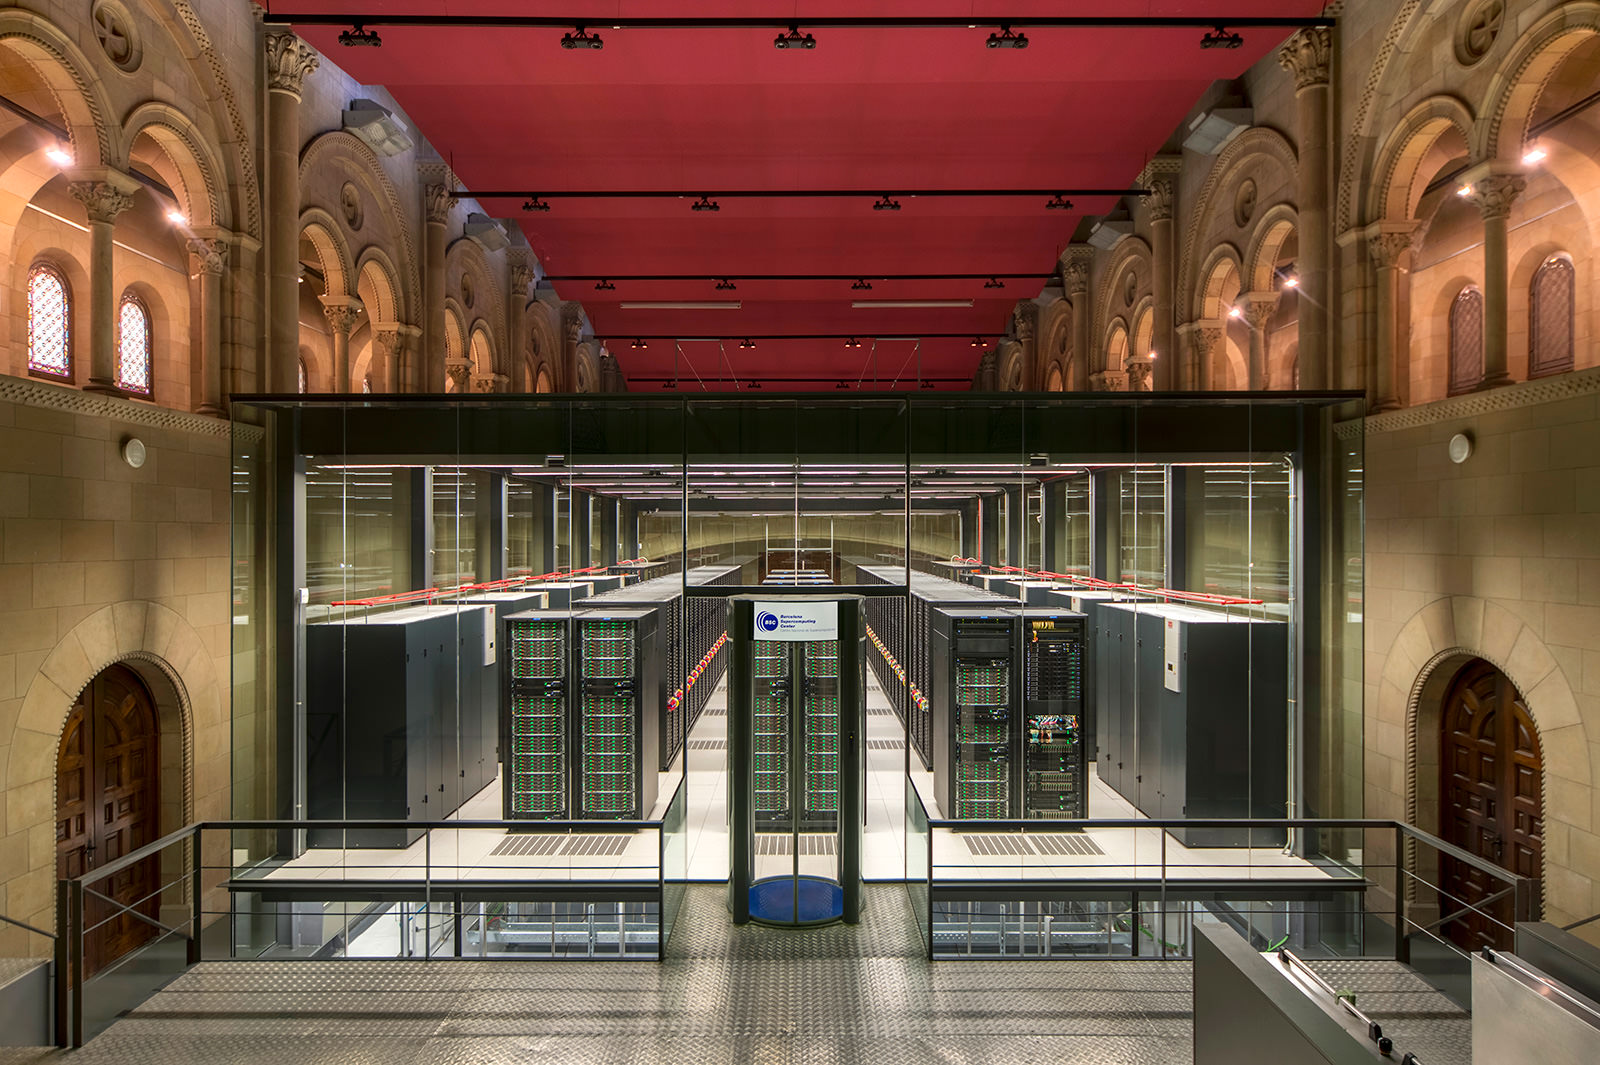
\includegraphics[width=5.5cm]{../figures/mare_nostrum.jpg}
\caption*{Mare nostrum supercomputer, Barcelona. Credits: bcs.es}
\end{figure}
\end{minipage}
}
%
\frame{
\frametitle{Remote sensing}
\begin{minipage}{0.48\linewidth}
\begin{itemize}
\item Another problem is that we cannot measure the physical parameters directly. We have to measure whatever the object is emitting:  
\begin{itemize}
\item [$\bullet$] Gravitational waves
\item [$\bullet$] Neutrinos
\item [$\bullet$] but mostly electromagnetic waves (\textbf{light})
\end{itemize}
\item This problem is tackled in more depth in another course: "Experimental Astrophysics: Remote Sensing", that will take place in the winter semester 2025/26.
\end{itemize}
\end{minipage}
\hfill
\begin{minipage}{0.48\linewidth}
\begin{figure}
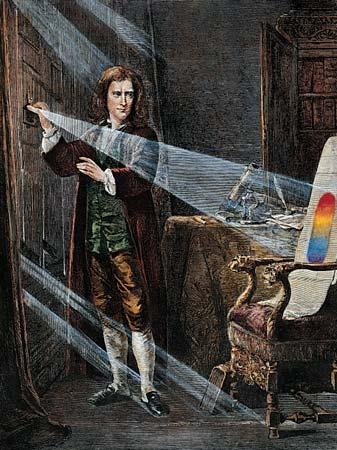
\includegraphics[width=4.5cm]{../figures/newton_prism.jpg}
\caption*{Engraving after a picture by J.A. Houston, ca. 1870. Courtesy of The Granger Collection, New York}
\end{figure}
\end{minipage}
}
%
\frame{
\frametitle{Gravitational wave astronomy}
\begin{minipage}{0.48\linewidth}
\begin{itemize}
\item Just like moving charges emit electromagntic waves, moving masses emit gravitational waves (GW)
\item They cause the space-time to fluctuate - The tiny variations in distance can be detected 
\item The LIGO experiment uses interferometry to detect tiny variations in the distance between two
perpendicular arms.
\item First successful detection: 2016. Nobel in 2017.
\end{itemize}
\end{minipage}
\hfill
\begin{minipage}{0.48\linewidth}
\begin{figure}
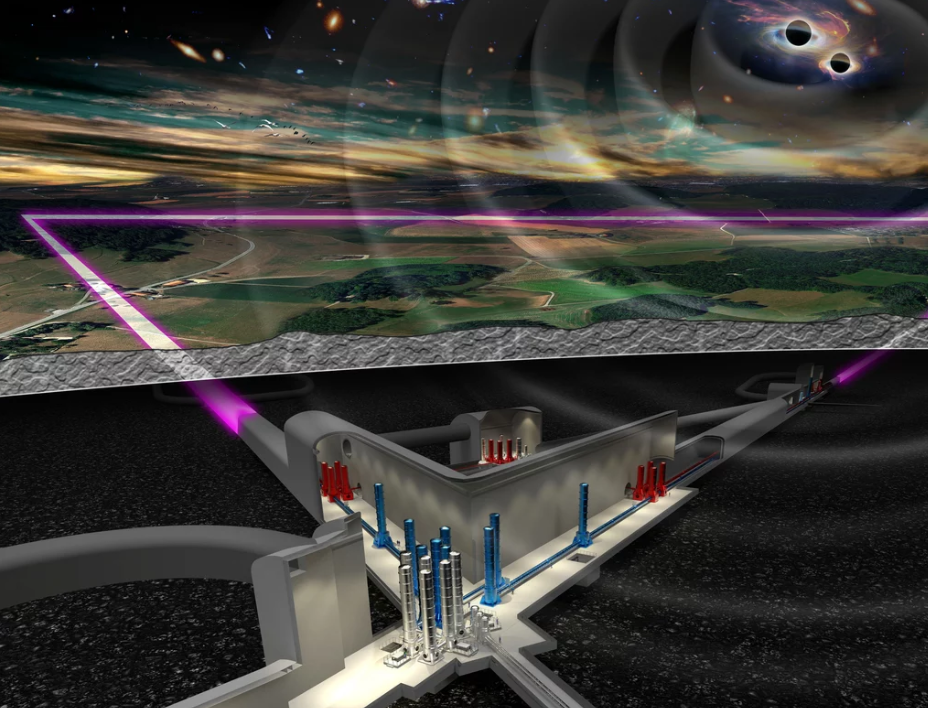
\includegraphics[width=6cm]{../figures/et.png}
\caption*{Future Einstein Telescope (artist impression). Credits: NIKHEF}
\end{figure}
\end{minipage}
}
%
\frame{
\frametitle{Neutrino astronomy}
\begin{itemize}
\item Existence of the neutrino first postulated by Pauli (1930) to conserve energy and momentum during $\beta$-decay. First detection by Reines \& Cowan (1956). Nobel in 1995.
\item Neutrinos are produced in the interior of stars as a consequence of nuclear reactions (i.e. \red{p-p chain})
\begin{center}
\begin{tcolorbox}[width=8cm,colback=tan]
$4 ^{1}\!H^{+} + 2 e^{-} \rightarrow ^{4}\!\!He^{2+} + \nu_e + \textrm{27.63 MeV}$
\end{tcolorbox}
\end{center}
\item Also produced during supernova explosions.
\item There is also the cosmic neutrino background: dates from 1 sec after the Big Bang. 
\item The cosmic microwave background, was produced some 380,000 years later.
\end{itemize}
}
%
\frame{
\frametitle{Solar Neutrino Problem}
\begin{minipage}{0.52\linewidth}
\begin{itemize}
\footnotesize{
\item According to the Standard Solar Model, the Sun's core has a temperature of about $T \approx 1.5\times 10^7$\,K.
\item At this temperature, the Sun should be producing a given number of neutrinos per second.
\item Experiments such as the Superkamiokande, detect only one third.
\item Does this mean that the temperature in the Sun's core is lower ? Is the Standard model wrong? Strong debate in the 90's.
\item In fact, we detect only a third because Superkamiolande detects only $\nu_e$, but as
neutrinos having \textbf{small mass}, they change flavours ($\nu_e$, $\nu_\tau$, $\nu_\mu$) as they travel - Neutrino oscillations! (Nobel prize in 2015).
}
\end{itemize}
\end{minipage}
\hfill
\begin{minipage}{0.47\linewidth}
\begin{figure}
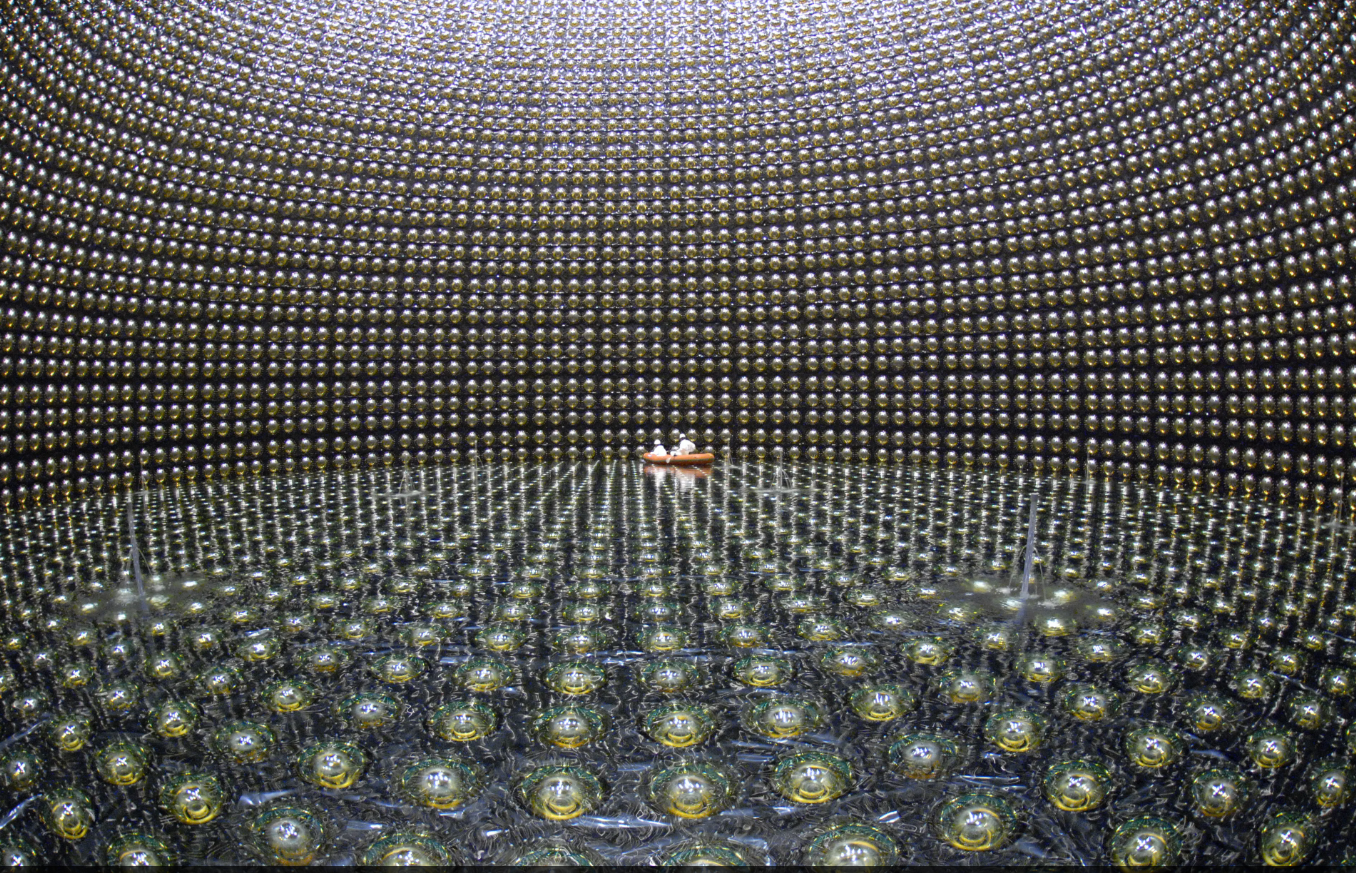
\includegraphics[width=6cm]{../figures/kamiokande.png}
\caption*{Credits Inst. Cosmic Ray Research, University of Tokyo}
\end{figure}
\end{minipage}
}
%
\section{Observing the stars}
\frame{
\frametitle{The light and the electromagnetic spectrum}
\begin{itemize}
\item The reason why we see \emph{anything} is because the light is coming from that object to our eyes or detectors (camera chip, etc..)
\item We see the planets and moons because they reflect the light, but we see th Sun and other stars because they \textbf{emit} the light.
\item That means there is energy generated in these objects that allows them to radiate.
\item \q{ Solve the following problem:} \emph{Total solar irradiance} (radiative energy per second per square meter at the top of the Earth's atmosphere) is 1361 W/m$^2$. How much energy does Sun produce per second? (Ask for any constants you need).
\end{itemize}
}
%
\frame{
\frametitle{The light and the electromagnetic spectrum}
\begin{itemize}
\item That means there is energy generated in these objects that allows them to radiate.
\item \q{ Solve the following problem:} \emph{Total solar irradiance} (radiative energy per second per square meter at the top of the Earth's atmosphere) is 1361 W/m$^2$. How much energy does Sun produce per second? (Ask for any constants you need).
\item Answer: 
\begin{equation}
\frac{dE}{dt} \equiv L_{\odot} = \mathcal{E}  4\pi d^2 = 1361 \rm{W m^{-2}} 4\pi (149 \times 10^9 \rm{m})^2 = 3.846\times 10^{26} \rm{W}
\end{equation}
\end{itemize}
}
%
\frame{
\frametitle{Effective temperature}
$3.846\times 10^{26} \rm{W}$ \q{is a lot of energy. What would roughly have to be the temperature of the Sun, so it would radiate this amount of energy?}
}
%
\frame{
\frametitle{Stefan-Boltzmann law}
\begin{itemize}
	\item The simplest way for us to relate the emitted energy to the temperature is through the Stefan-Boltzmann law. 
	\item The emissivity (emitted energy per unit surface in the outgoing direction) is equal to: 
	\begin{equation}
	\mathcal{E}^{em} = \sigma T^4
	\end{equation}
	\item Then, the luminosity (emitted energy per second) of such object is: 
	$L = 4\pi R^2 \sigma T^4$. 
	\item If you substitute the numbers, you will get $T=5777\,\rm{K}$.
	\item \q{What temperature would this be?}
	\item \q{What does this question even mean?}
\end{itemize}
}
%
\frame{
\frametitle{Departures from the ideal case}
We made a series of approximations in the process of inferring this temperature. 
\begin{itemize}
\item First we assumed that the solar radiance is constant in time (\emph{excellent approximation})
\item Then we assumed that the emission is isotropic (\emph{this is not a good approximation but see below})
\item Then we assumed that the solar surface is homogeneous (\emph{on small scales it is not, but let's discuss this for a while})
\item Finally, we assumed that the Sun emits like a blackbody to infer the called \text{effective temperature} - 5777K. 
\item \q{Let's discuss a bit what this concept means - 5 mins}
\end{itemize}
}
%
\frame{
\frametitle{Real situations}
\begin{minipage}{0.52\linewidth}
The Sun (and other stars) depart severely from these assumptions:
\begin{itemize}
	\item Stars are inhomogeneous in all 3 dimensions (especially radially).
	\item They emit non-Plankian spectra, in a generally anisotropic manner
	\item And they also change on scales from seconds to billions of years. 
	\item \textbf{This course is about all these aspects}
\end{itemize}
\end{minipage}
\hfill
\begin{minipage}{0.46\linewidth}
\begin{figure}
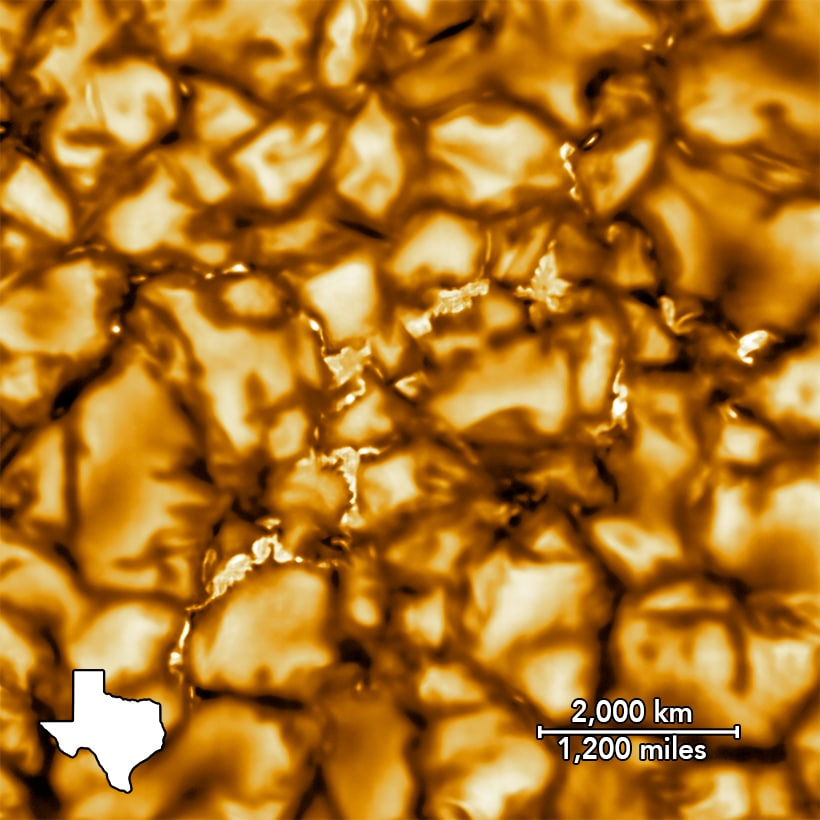
\includegraphics[width=5cm]{../figures/dkist1.jpg}
\caption*{Credits: NSO/AURA/NSF/DKIST}
\end{figure}
\end{minipage}
}
%
\frame{
\frametitle{The concept of stellar atmosphere}
\begin{itemize}
\item Energy is generated in the cores of stars and transported outwards (in multiple ways)
\item As we move away from the stellar center - the medium becomes less opaque, at some point the photons can escape the star. Then they contribute to the total stellar luminosity that we ultimately detect.  
\item The \sepia{layer} of the last emission is referred to as $\tau=1$ layer, where $\tau$ is the so called \textbf{optical depth}.
\item As the stars are made of plasma - we don't have an obvious surface. $\tau=1$ layer serves as a loose definition of a solar surface (observationally).
\item Next week, we will describe a star using equations of stellar structure - we will again have to make a definition of solar surface.
\end{itemize}
}
%
\frame{
\frametitle{The concept of stellar atmosphere}
\begin{minipage}{0.52\linewidth}
\begin{itemize}
\item The physical location of $\tau=1$ depends on the density of the medium and how the photon interacts with the medium - \textbf{described by the opacity}.
\item Solar plasma has different opacity at different wavelengths - photosphere has different physical location.
\item Also, when we look at the Sun under different angles, we see different depths. 
\item This is the so called limb-darkening. 
\end{itemize}
\end{minipage}
\hfill
\begin{minipage}{0.47\linewidth}
\begin{figure}
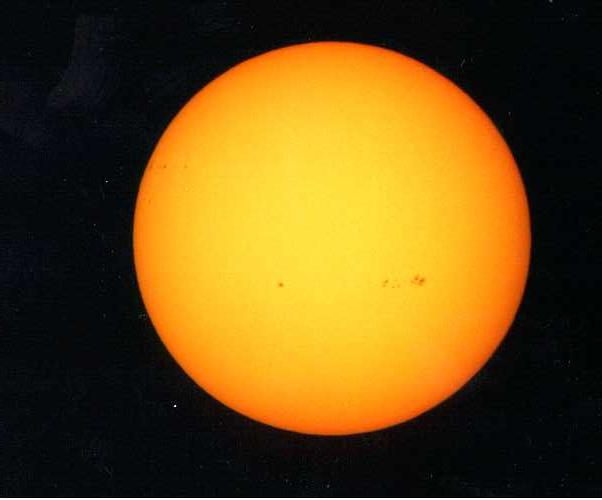
\includegraphics[width=6cm]{../figures/sun_orange.jpg} 
\end{figure}
\end{minipage}
}
%
\frame{
\frametitle{Why study the stellar atmospheres?}
\begin{itemize}
\item The stellar light gives us direct information about the stellar surface (the photosphere).
\item \q{Are there ways to probe the stellar interior? Can the stellar atmosphere help?}
\end{itemize}
}
%
\frame{
\frametitle{Why study the stellar atmospheres?}
\begin{itemize}
%\item The stellar light gives us direct information about the stellar surface (the photosphere).
\item \q{Are there ways to probe the stellar interior? Can the stellar atmosphere help?}
\item Stellar structure determines the structure of the atmosphere, and $T_{\rm eff}$.
\item Stellar atmosphere oscillates because of the processes in stellar interior. 
\item At the surface, we measure the magnetic fields generated in the interior. 
\item Neutrinos produced in the core leave the star directly. 
\item \textbf{The structure of the whole star leaves an observable imprint on its surface.}
\end{itemize}
}
%
\frame{
\frametitle{Understanding the stars}
\begin{itemize}
\item \textbf{The structure of the whole star leaves an observable imprint on its surface.}
\item We measure these observable imprints. 
\item We can observe \emph{a lot} of stars - so we can have accurate statistics. 
\item \textbf{We devise theoretical models that try to describe the stellar structure and the evolution and compare the outputs of these models both to the measurable properties of individual stars and to the statistical distributions.}
\end{itemize}
}
%
\section{Stellar colors}
%
\frame{
\frametitle{Luminosity vs the color}
\begin{itemize}
\item Effective temperature describes the total luminosity of the star.
\item We used a blackbody to approximate solar \emph{surface}.
\item Now, different temperatures imply different colors (i.e. different spectral distributions).
\begin{figure}
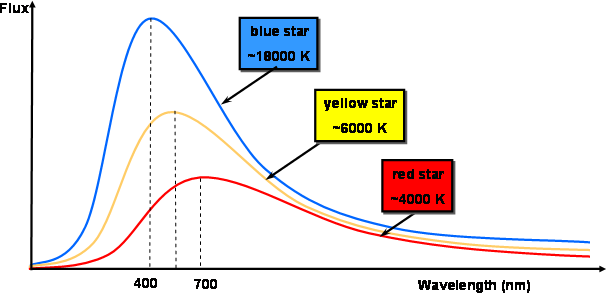
\includegraphics[width=7.5cm]{../figures/bb_curves.png}
\caption{Planck curves for blackbodies of different temperatures. Credits: University of Swinburne}
\end{figure}
\end{itemize}
}
%
\frame{
\frametitle{A side quest}
\begin{itemize}
\item \q{Can someone convince me that a star \textbf{cannot} be a blackbody? - 2-3 mins}
\end{itemize}
}
%
%
\frame{
\frametitle{Stars are not black bodies!}
\begin{itemize}
\item Star needs to transport energy outwards. For that a gradient of temperature is needed - not a blackbody. 
\item \q{Harder question is can stellar photosphere be a blackbody?}
\item In theory - yes, no fundamental law would be broken if it was. 
\item In practice - it can't. Different wavelengths \emph{always} have different opacities and thus sample different depths.
\end{itemize}
}
%
\frame{
\frametitle{Solar spectrum is NOT a blackbody spectrum}
\begin{figure}
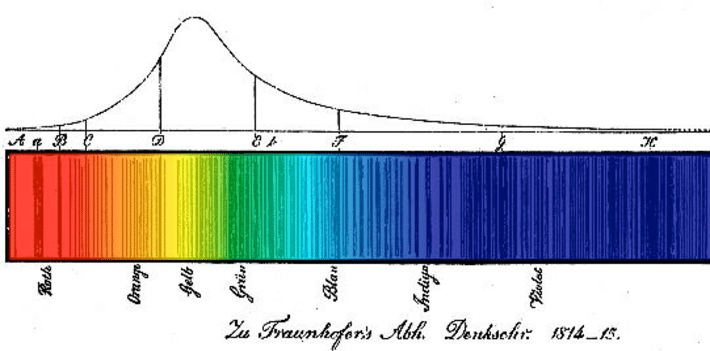
\includegraphics[width=10cm]{../figures/fraunhofer_spectrum.png}
\caption*{Credits: Fraunhofer (1814)}
\end{figure}
\begin{itemize}
\item Wollastone (1802) and Fraunhofer (1814) discovered dark lanes in the solar spectrum,
\item These lines represent loss of light at specific wavelengths - solar atmosphere is much more opaque at these wavelengths. \q{Why?}
\end{itemize}
}
%
%
\frame{
\frametitle{Solar spectrum is NOT a blackbody spectrum}
\begin{figure}
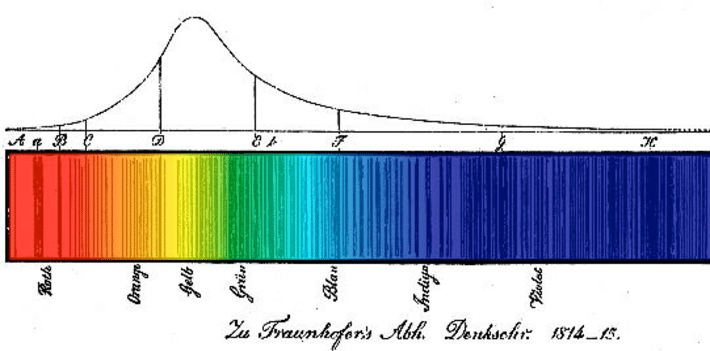
\includegraphics[width=6cm]{../figures/fraunhofer_spectrum.png}
\caption*{Credits: Fraunhofer (1814)}
\end{figure}
\begin{itemize}
\item These lines represent loss of light at specific wavelengths - solar atmosphere is much more opaque at these wavelengths. \q{Why?}
\item Kirchoff and Bunsen (1860's) related them to chemical elements. 
\item Birth of quantum mechanics: Bohr's model can explain hydrogen lines. \textbf{Energy jumps between discrete energy levels}.
\item Discovery of Helium by Janssen (1868) in the solar spectrum.
\end{itemize}
}
%
%
\frame{
\frametitle{Planck Law}
\begin{itemize}
\item Kirchoff (again) reckognized the importance of an universal law that connects emission and absorption properties of a medium in an equilibrium state. - \emph{"... It is of utmost importance to derive this law theoretically"}. 
\item We had some pieces - Stefan-Boltzmann law that we just talked about...
\item ... Then we had Wien's law: Emission of bodies of different temperature peaks at different wavelengths (colors).
\item People also experimentally captured the dependence $B(T)$, where $B$ is some ``brightness" or essentially luminosity.
\item \emph{Interesting:} Both Boltzmann and Wien (as well as Rayleigh and later Jeans) derived the corresponding laws theoretically. \q{Do you know how?}
\item Recommendation: ``Theoretical Concepts in Physics'' (Malcom Longair, 2020, Cambridge)
\end{itemize}
}
%
\frame{
\frametitle{Planck Law}
\begin{minipage}{0.5\linewidth}
\begin{itemize}
\item Finally, Planck derived this law theoretically. 
\item After that, multiple other approaces to derivation were made (for example one by Bose and Einstein).
\begin{equation}
B(\lambda, T) = \frac{2hc^2}{\lambda^5} \frac{1}{e^{hc/\lambda k T} - 1}
\end{equation}
\item This equation describes the \emph{intensity} of the light in a state where photons are in equilibrium. 
\end{itemize}
\end{minipage}
\hfill
\begin{minipage}{0.49\linewidth}
\begin{figure}
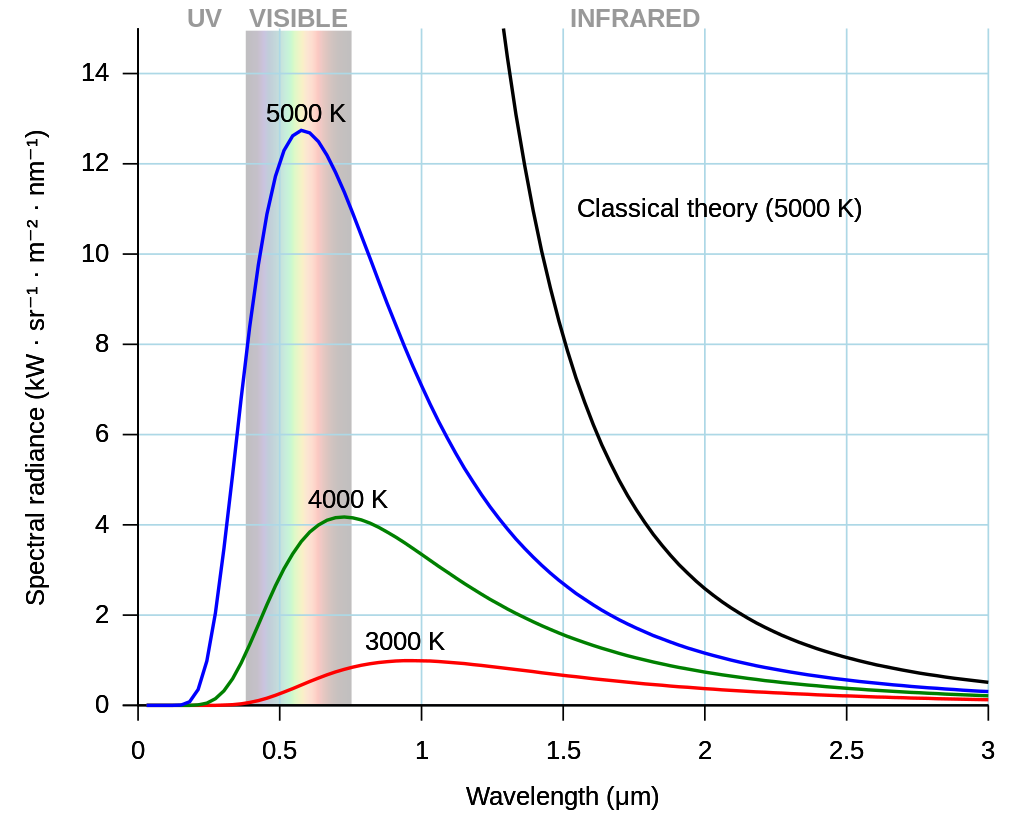
\includegraphics[width=8cm]{../figures/b_b2.png}
\caption*{Planck curves for few different temperatures. Credits: Wikipedia}
\end{figure}
\end{minipage}
}
%
%
\frame{
\frametitle{Solar spectrum is NOT a blackbody spectrum}
\begin{figure}
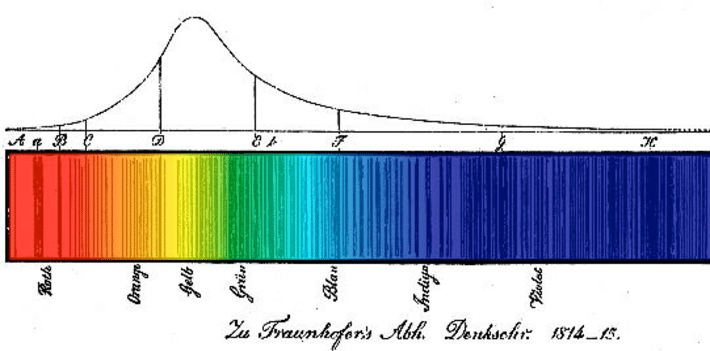
\includegraphics[width=6cm]{../figures/fraunhofer_spectrum.png}
\caption*{Credits: Fraunhofer (1814)}
\end{figure}
\begin{itemize}
\item These lines represent loss of light at specific wavelengths - solar atmosphere is much more opaque at these wavelengths. \q{Why?}
\item Kirchoff and Bunsen (1860's) related them to chemical elements. 
\item Birth of quantum mechanics: Bohr's model can explain hydrogen lines. \textbf{Energy jumps between discrete energy levels}.
\item Discovery of Helium by Janssen (1868) in the solar spectrum.
\end{itemize}
}
%
\frame{
\frametitle{Today we can do better than 200 years ago ...}
\begin{figure}
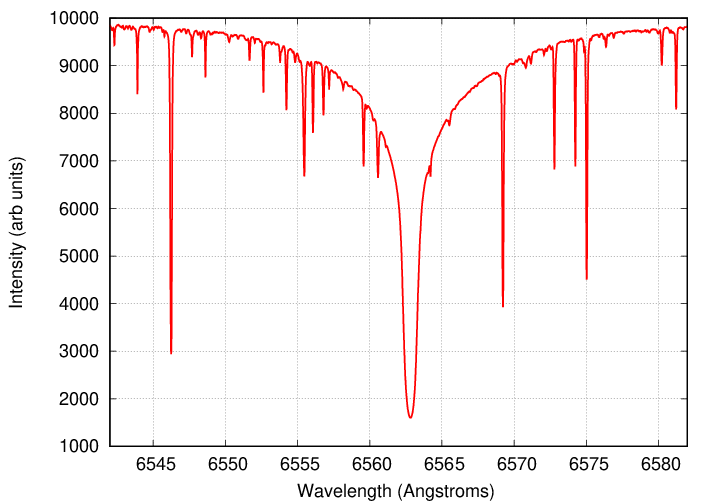
\includegraphics[width=8cm]{../figures/sun_halpha_a.png}
\caption*{H$\alpha$ spectral line in solar spectrum: notice all the weak spectral lines around!}
\end{figure}
}
%
\frame{
\frametitle{And we can do the same for other stars.}
\begin{figure}
\begin{tabular}{cc}
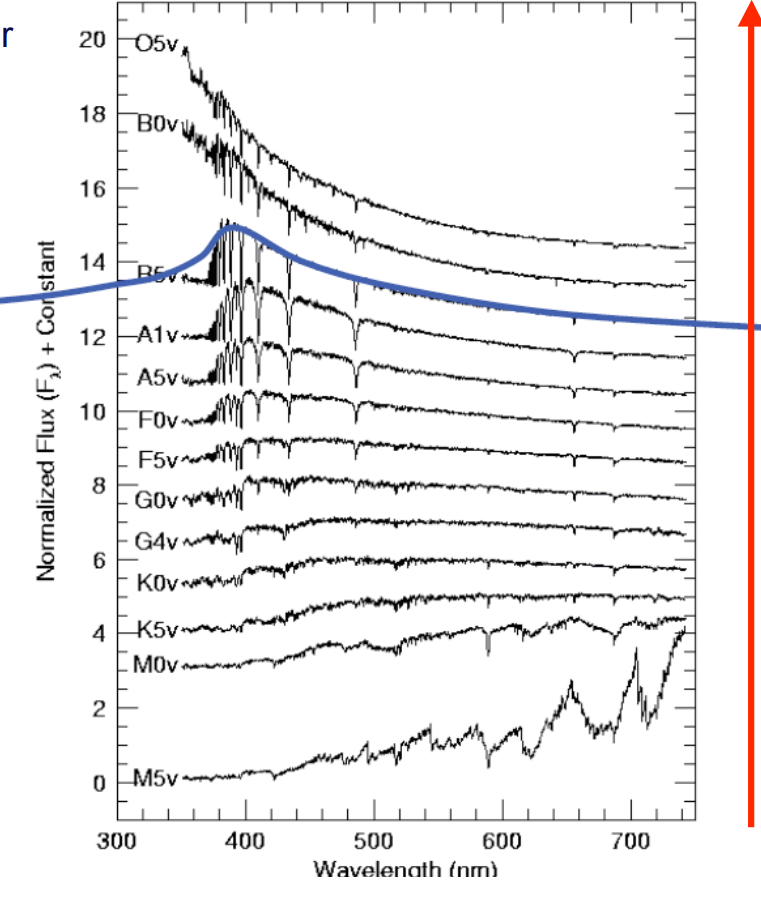
\includegraphics[width=9cm]{../figures/spectra_stars.png}
\end{tabular}
\caption*{Credits: Adam Burrows, Princeton}
\end{figure}
}
%
%
\frame{
\frametitle{And we can do the same for other stars.}
\begin{minipage}{0.45\linewidth}
\q{What is the fundamental parameter that determines the shape of the spectrum and the absence/presence of spectral lines?}
\end{minipage}
\hfill
\begin{minipage}{0.54\linewidth}
\begin{figure}
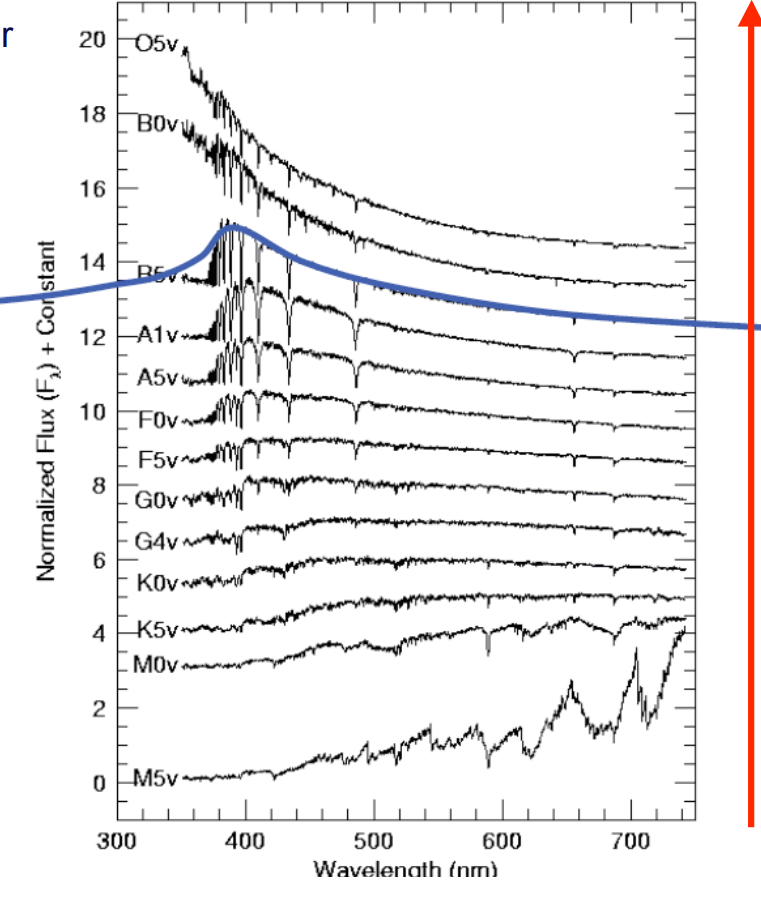
\includegraphics[width=6cm]{../figures/spectra_stars.png}
\caption*{Credits: Adam Burrows, Princeton}
\end{figure}
\end{minipage}
}
%
%
\frame{
\frametitle{And we can do the same for other stars.}
\begin{minipage}{0.45\linewidth}
\q{What is the fundamental parameter that determines the shape of the spectrum and the absence/presence of spectral lines?}

It is the temperature! It determines the ionization and excitation of the particles and thus their absorption/emission properties.
\end{minipage}
\hfill
\begin{minipage}{0.54\linewidth}
\begin{figure}
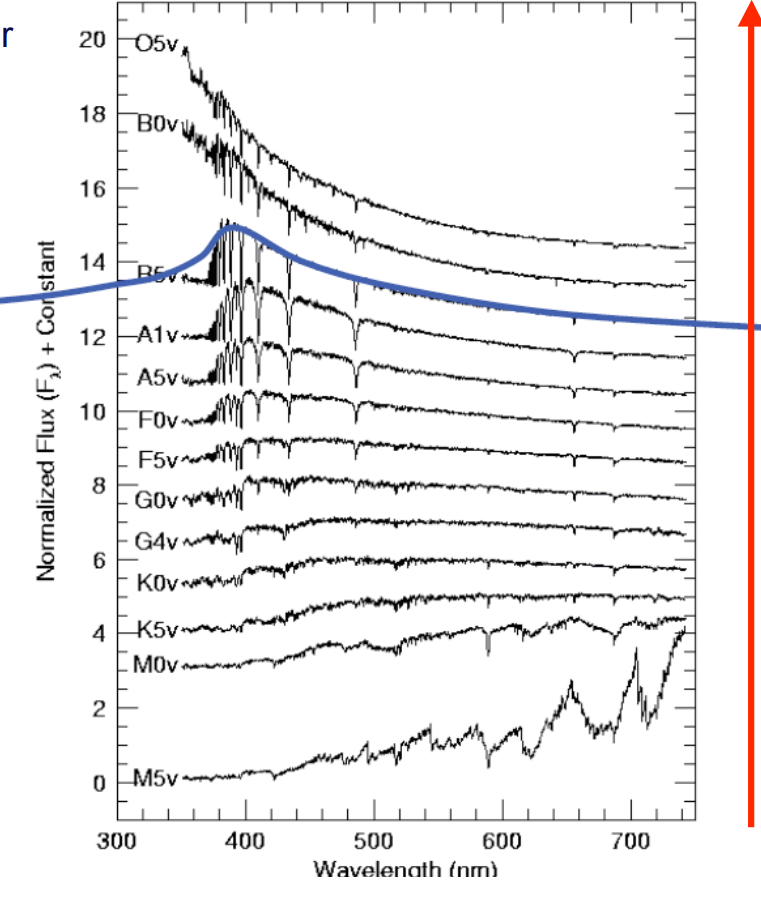
\includegraphics[width=6cm]{../figures/spectra_stars.png}
\caption*{Credits: Adam Burrows, Princeton}
\end{figure}
\end{minipage}
}
%

\frame{
\frametitle{The Harvard Spectral Classification}
\begin{minipage}{0.48\linewidth}
\begin{tabular}{cc}
Class & \red{T$_{\rm eff}$} [K] \\
\hline
O & $\ge$ 30000 \\
B & 10000-30000 \\
A & 7500-10000 \\
F & 6000-7500 \\
G & 5000-6000 \\
K & 3000-5000 \\
M & 2000-3000 
\end{tabular}
\end{minipage}
\hfill
 \begin{minipage}{0.48\linewidth}
\begin{figure}
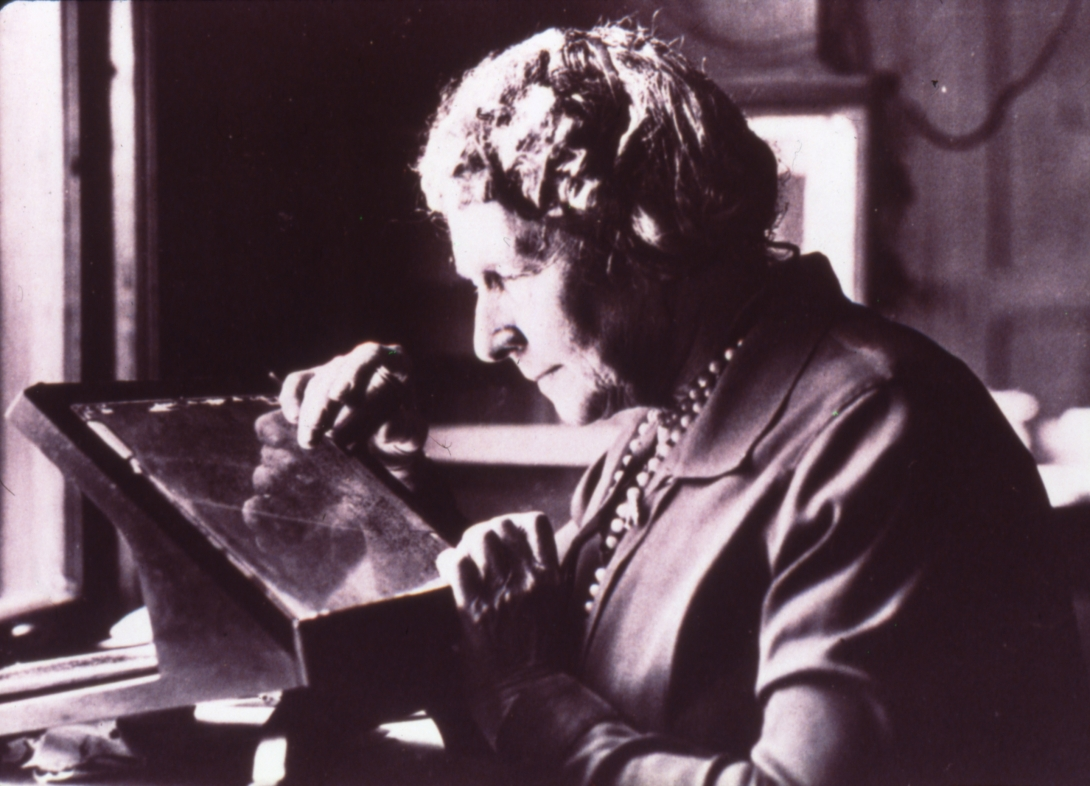
\includegraphics[width=6cm]{../figures/ajc.jpg}
\caption*{Annie Jump Cannon. Credits: Library of Congress, US}
\end{figure}
\end{minipage}
}
%
\frame{
\frametitle{HR diagram: basics}
\begin{minipage}{0.48\linewidth}
\begin{itemize}
\item There are three groups of stars.
\item For one (main sequence) the color and brightness are somewhat correlated.
\item Other is very hot but faint - white dwarves
\item The last is cool but bright - (red) giants (there are also other giants).
\item It will turn out these are \emph{phases} in stellar evolution.
\end{itemize}
\end{minipage}
\hfill
\begin{minipage}{0.48\linewidth}
\begin{figure}
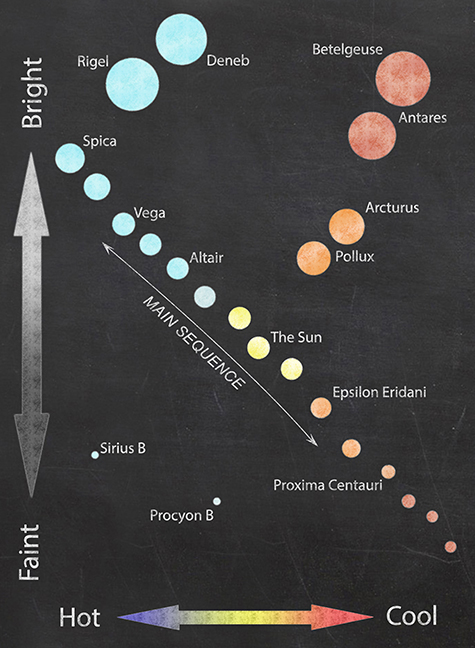
\includegraphics[width=5.2cm]{../figures/hr_simple.jpg}
\caption*{Credits: the Open University}
\end{figure}
\end{minipage}
}
%
%
\frame{
\frametitle{HR diagram: basics}
\begin{minipage}{0.48\linewidth}
\begin{itemize}
\item It will turn out these are \emph{phases} in stellar evolution.
\item We \textbf{can't} observe stars as they evolve and age.
\item But we can observe a lot of stars and try to infer things. 
\item It is like aliens observed us very briefly: they would need some time that small, weak humans are a first stage in a lifetime of a human being.
\end{itemize}
\end{minipage}
\hfill
\begin{minipage}{0.48\linewidth}
\begin{figure}
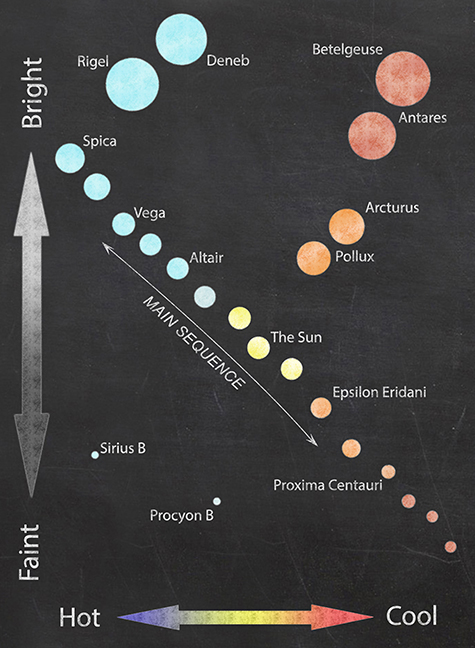
\includegraphics[width=5.2cm]{../figures/hr_simple.jpg}
\caption*{Credits: the Open University}
\end{figure}
\end{minipage}
}
%
%
\frame{
\frametitle{HR diagram: questions}
\begin{minipage}{0.48\linewidth}
\begin{itemize}
\item Why are the color and the brightness of the stars on the main sequence correlated?
\item In which order these evolutionary stages take place?
\item What determines when and how the star changes between these stages?
\item What are the fundamental differences between these phases?
\end{itemize}
\end{minipage}
\hfill
\begin{minipage}{0.48\linewidth}
\begin{figure}
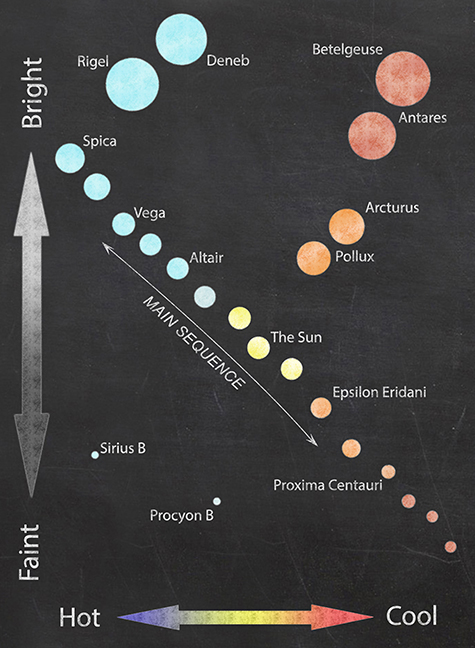
\includegraphics[width=5.2cm]{../figures/hr_simple.jpg}
\caption*{Credits: the Open University}
\end{figure}
\end{minipage}
}
%
\frame{
\frametitle{How can we infer other stellar parameters?}
\begin{itemize}
	\item We saw that we can estimate luminosity from the apparent brightness (irradiance) and distance. 
	\item And that we can infer the effective temperature from the color.
	\item Combined, these two give us the radius (an estimate of).
	\item \q{Write down the equations again if necessary}.
	\item What about the mass? Physical composition? Magnetic field? Rotation rate?
\end{itemize}
}
%
\frame{
\frametitle{Stellar masses}
\begin{minipage}{0.48\linewidth}
\begin{itemize}
\item Are extremely important, yet extremely hard to infer.
\item The only accurate opportunity to infer the mass is to observe the star in a dynamical interaction.
\item For example in a binary system. 
\item These binary stars are very important, a big fraction of the stars are in binary (or multiple systems).
\item The stars can also interact with each other. 
\end{itemize}
\end{minipage}
\hfill
\begin{minipage}{0.48\linewidth}
\begin{figure}
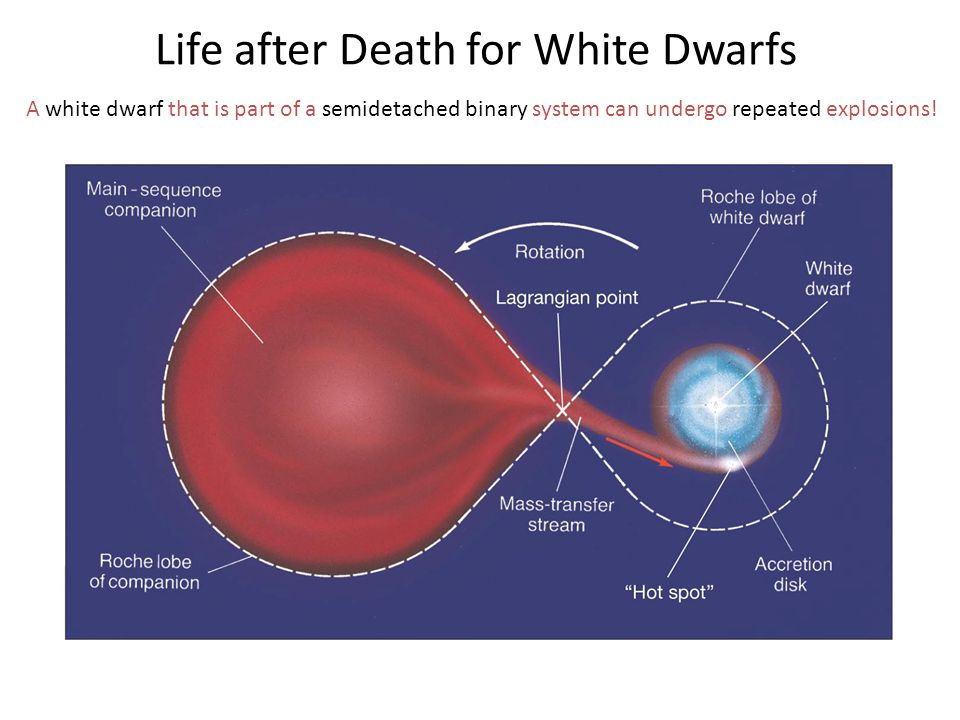
\includegraphics[width=6cm]{../figures/roche_lobe.jpg}
\end{figure}
\end{minipage}
}
%
\frame{
\frametitle{Element abundances in the Universe }
\begin{minipage}{0.48\linewidth}
\begin{itemize}
\item Most of these elements were generate in stars. 
\item But they also have implications for generation and evolution of other stars? 
\item \q{Let's have a relaxed discussion on importance of heavier elements.}
\end{itemize}
\end{minipage}
\hfill
\begin{minipage}{0.48\linewidth}
\begin{figure}
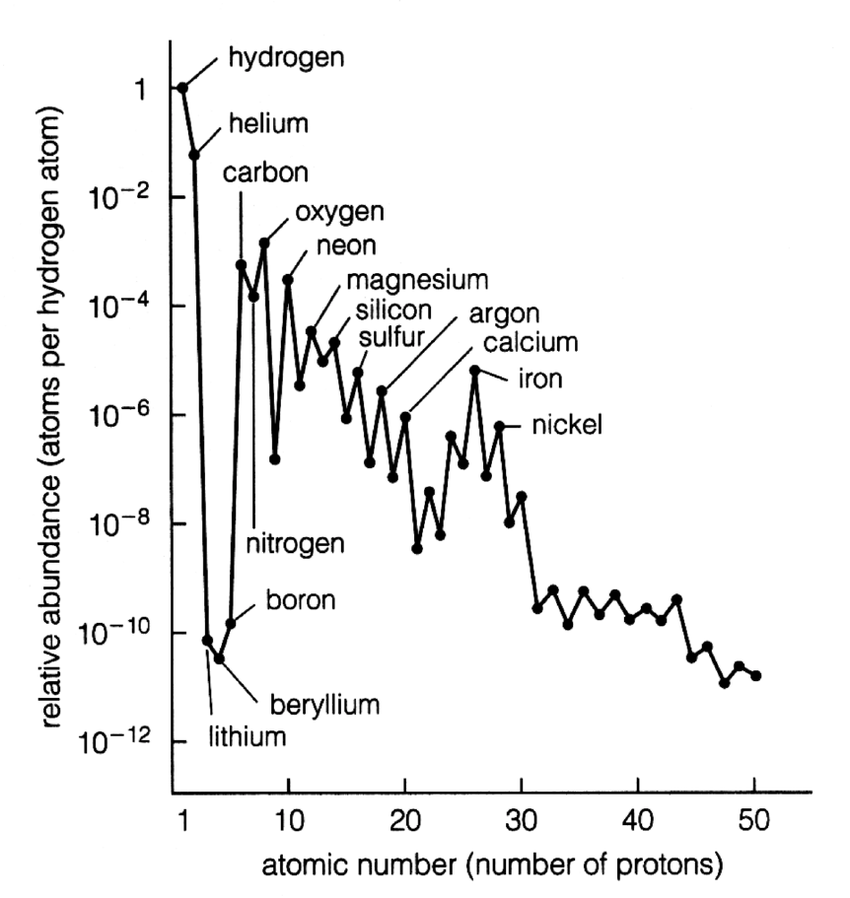
\includegraphics[width=6cm]{../figures/The-relative-abundances-of-elements-in-the-universe-after-Goldschmidt-1938.png}
\caption*{Credits: Goldschmidt 1938}
\end{figure}
\end{minipage}
}
%
\frame{
\frametitle{These abundances are inferred from the spectra}
\begin{minipage}{0.48\linewidth}
\begin{itemize}
\item Determination of the Silicon Abundance by fitting the solar spectra
\item \sepia{Dots}: observations; \sepia{dashed/solid}: low/high Silicon abundance.
\end{itemize}
\end{minipage}
\hfill
\begin{minipage}{0.48\linewidth}
\begin{figure}
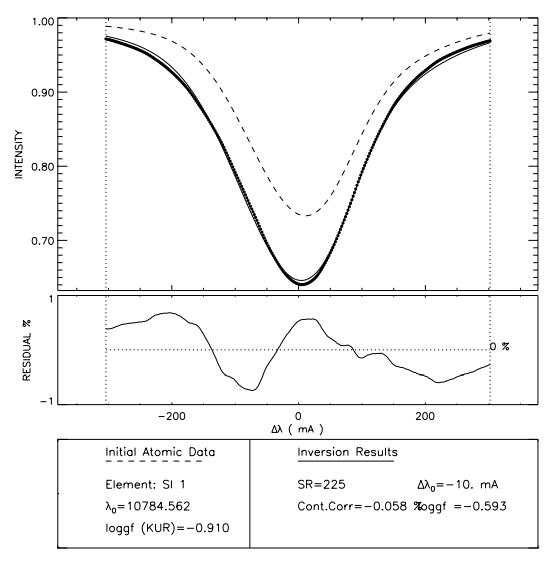
\includegraphics[width=6cm]{../figures/abundance_si.png}
\caption*{Credits: Borrero et al. 2003}
\end{figure}
\end{minipage}
}
%
%
\frame{
\frametitle{Question to think about}
\begin{itemize}
	\item We said that the effective temperature of the Sun is $5777$\,K.
	\item We also said that this temperature is not constant, but must be increasing inward, in order to drive energy flux outward.
	\item \q{What is the temperature in the core?}
	\item \q{What is the source of energy?}
\end{itemize}
}
%
\frame{
\frametitle{Answer}
\begin{itemize}
	\item The temperature at the core is $\approx 1.5\times 10^7$\,K. And the source of energy is nuclear fusion of $H$ in $He$. 
	\item How do we know? It took us some time. 
	\item First one to even think about this was Eddington. (Maybe check \href{https://arxiv.org/pdf/2111.02096.pdf}{this} paper by H. Kragh).
	\item The previous idea was graviational contraction. 
	\item The temporal scale for such a process is the \textbf{Kelvin-Helmholtz timescale}.
\end{itemize}
}
%
\frame{
\frametitle{Kelvin-Helmholtz timescale}
\begin{itemize}
	\item Let's do an order of magnitude estimation:
	\begin{equation}
	t_{\rm KH} = \frac{GM^2}{RL}
	\end{equation}
	\item For the Sun this amounts to 30 million years. 
	\item We knew back then already that Earth is billions of years old. 
	\item It had to be something else!
	\item There will be a master course in German on ``Fluid Dynamics'' by Prof. Antonio Ferriz Mas, starting in May - keep an eye out! 
	\item See you on ???? \q{Make a plan if we hve not already: Online / in person?}
\end{itemize}
}
\end{document}



